\chapter[Background]{Background\footnote{Contains text \& images from the author's Minor Thesis `Business Ideation for \gls{ble}', derived from this thesis' work}} \label{2Back}

This chapter aims at providing a succinct background necessary to understanding the rest of the thesis report. Readers are directed to the references for a comprehensive overview. Section \ref{OverviewBLE} provides an overview of the BLE technology required for following this document. Description of Contiki \gls{os} and literature involving the process of porting of Contiki \gls{os} to a hardware platform are presented in section \ref{OverviewContiki}. This chapter ends with presenting the aspects related to the 802.15.4 protocol utilized in this project.


\section{Overview of \texorpdfstring{\acrlong{ble}}{Bluetooth Low Energy}} \label{OverviewBLE}

\acrfull{ble} is a relatively new low power standard incorporated in Bluetooth Core Specification Version 4.0 released by Bluetooth \gls{sig} in 2010\cite{CoreSpec4.0}. This wireless personal area network is marketed as Bluetooth Smart the Bluetooth \gls{sig}. Devices containing only BLE hardware are \emph{single mode} devices, whereas devices containing both classic Bluetooth and BLE are known as \emph{dual mode} devices.   

\gls{ble} was designed by Bluetooth \gls{sig} from the ground up, which helped it achieve certain design goals. These design goals for this wireless personal area network were \emph{low cost, worldwide operation, short range, robustness} and \emph{low power}\cite{Heydon2012}. One most important differentiating factors that has made BLE so successful is the standardization by Bluetooth SIG, facilitating its inclusion in consumer devices and enabling communication across different vendors. In 2013, over 85\% consumer electronic devices supported BLE, making it the de facto standard for low power wireless communication in these devices\cite{Martin2014}. BLE is adopted for various control, notification and monitoring applications, especially in the healthcare, fitness, security and home entertainment industry. 

%\subsection{Design objectives of \gls{ble}}
%
%\paragraph{Low Power} \gls{ble} aims to use a tiny batteries such as button cell to keep a device operating for months to years. To achieve this goal, \gls{ble} was optimized to communicate small amounts of data, such as the states of devices. Also \gls{ble} is optimized to have lower peak power requirements, which allows use of button cells to be used with \gls{ble} devices.
%\paragraph{Worldwide Operation}
%For a technology to be adopted, it is important that there is uniform conformity to the regulations around the world. The 2.4 \si{\GHz} \gls{ism} radio band is the only one available license free worldwide. The technology to develop wireless devices in this band is mature making it the suitable radio band for \gls{ble}.
%\paragraph{Short Range}
%\gls{ble} was designed to be for personal area network like Classic Bluetooth, which means that it is not a network to work with a cellular base station network. This design criterion goes hand in hand with \emph{low power}.
%\paragraph{Low Cost} Lower power requirements mean that the batteries in \gls{ble} devices need to smaller and have to be replaced less frequently, both resulting in a reduction of cost for both the manufacturer and the customer. The use of the \gls{ism} band for communication levels removes the licensing entry barrier for start-ups to develop \gls{ble} devices. \gls{ble} embraces simplicity in its pursuit to lower the cost. \gls{ble} supports only single-hop communication in a star network, which reduces the memory and processor requirement for supporting the protocol. Simplicity was the key factor for the choosing of \gls{gfsk} as the modulation scheme for \gls{ble} to result in low cost, simple implementation of the radio in the \glspl{ic} for \gls{ble}. 
%\paragraph{Robustness} The 2.4~\si{\GHz} space is crowded with devices communicating with various standards as well as spurious noise making the robustness a key criteria in developing \gls{ble} standard. \gls{ble} uses a multi-channel hopping mechanism called \gls{afh} to detect, avoid and recover from interference. In addition to \gls{afh}, \gls{ble} uses \gls{crc} to detect and recover from bit-errors due to background noise.

\subsection[\texorpdfstring{\gls{ble}}{BLE} Network Architecture]{\texorpdfstring{\gls{ble}}{BLE} Network Architecture\cite{BLE101}}

\begin{table}[htbp]
\begin{center}
\vspace{-10pt}
\setlength{\extrarowheight}{1.5pt}
\begin{tabular}{|m{2.5cm}|m{1.2cm}|m{11.4cm}|}
\hline
\multicolumn{ 2}{|c|}{\textbf{State}} & \textbf{State Description} \\ \hline
\multicolumn{ 2}{|c|}{Standby} & Does not transmit or receive packets, usually sleeping \\ \hline
\multicolumn{ 2}{|c|}{Advertising} & Broadcasts advertisement packets in  advertising channels \\ \hline
\multicolumn{ 2}{|c|}{Scanning} & Looks for advertisement packets, across advertising channels \\ \hline
\multicolumn{ 2}{|c|}{Initiating} & Initiates connection to advertiser to get Master role \\ \hline
\multicolumn{ 1}{|m{2.0cm}|}{\hspace{42pt} \mbox{Connection}} & Master & Communicates with device(s) in the \emph{slave} role, defines configuration of the connection \\ \cline{ 2- 3}
\multicolumn{ 1}{|l|}{} & Slave & Communicates with a single device in \emph{master} role \\ \hline
\end{tabular}
\end{center}
\vspace{-12pt}
\caption{Possible states of a BLE device}
\vspace{-6pt}
\label{tbl:BLEstates}
\end{table}

Table \ref{tbl:BLEstates} shows the possible states of a BLE device and figure \ref{fig:Roles} illustrates the ways in which these states can change. The standby role is universally supported across all BLE devices and the other roles are present in device according to their configuration. For example, a device with only a radio transmitter can alternate between the advertising and standby state, usually called an \emph{advertiser}. Similarly a \emph{scanner} can just receive BLE packets.

\begin{wrapfigure}{r}{0.55\textwidth}
\centering
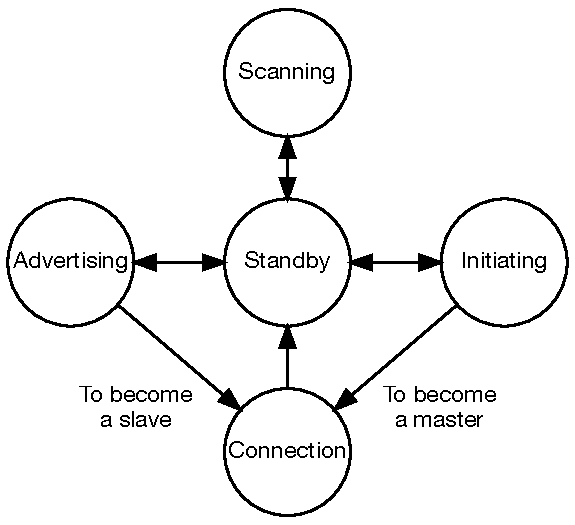
\includegraphics{Roles.pdf}
\caption{State diagram of BLE states}
\label{fig:Roles}
\vspace{-10pt}
\end{wrapfigure}

A connection can be formed between two BLE devices, with the master node reaching from the initiating state and the slave node from the advertising state. This master and slave roles follows an asymmetric design philosophy. A slave is a simple device that can be connected with at most one master at a time and are usually single purpose devices. A master on the other hand is a more complex device which is responsible for coordinating the connections and activities of all the slaves connected to it. A master is usually a multi-purpose device such as a mobile phone, tablet or a laptop. A master connected with multiple slaves employs a star topology. \gls{ble} only supports single hop communication, meaning that a master cannot communicate with a master and a slave cannot communicate with a slave. An example of a BLE network is shown in figure \ref{fig:TopoBLE}. Here a master can be seen connected to multiple slaves. The bidirectional continuous lines show data communicated in both directions when in a connection. The dashed lines show the data from the advertisements being sent broadcast. A master or slave can be an advertiser simultaneously as seen in the figure \ref{fig:TopoBLE}. Note that in this figure, since the advertisers are at the two ends, their signals are not able to reach both the master and the scanner device.

\begin{figure}[h]
\centering
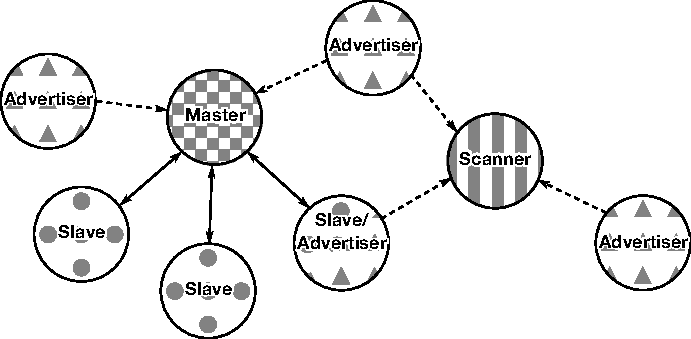
\includegraphics{TopologyBLE.pdf}
\caption{An example of BLE topology}
\label{fig:TopoBLE}
\vspace{-10pt}
\end{figure}

%\begin{figure}[h] %{r}{0.51\textwidth}
%%\vspace{-15pt}
%  \begin{center}
%	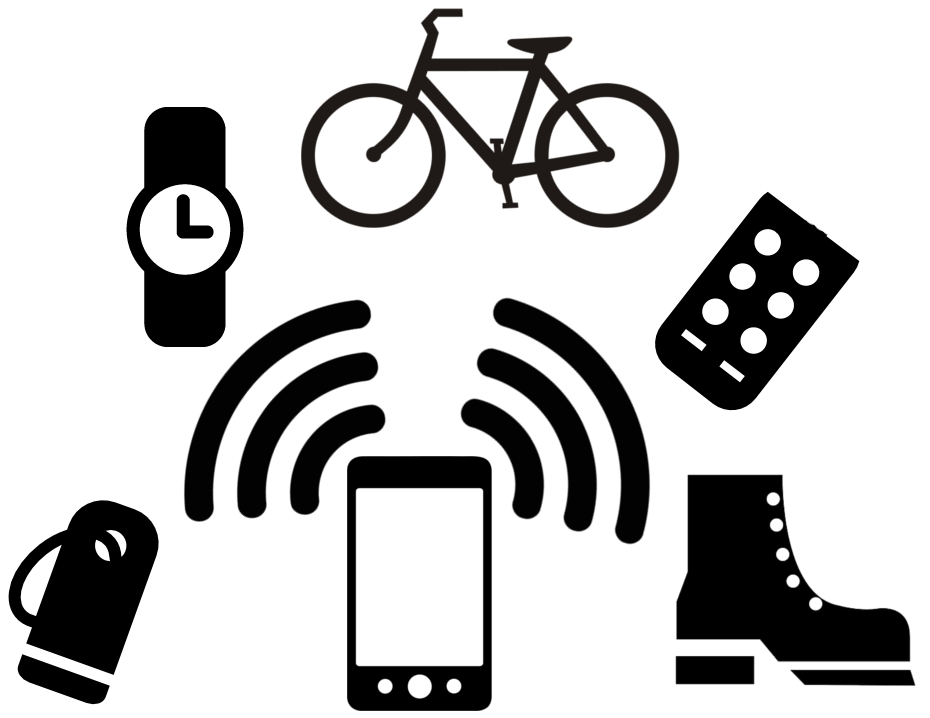
\includegraphics[width=0.49\textwidth]{devicesBLE}
%  \end{center}
%\caption{Typical BLE network}
%%\vspace{-10pt}
%\label{devicesBLE}
%\end{figure}

\section[\texorpdfstring{\gls{ble}}{BLE} Stack Overview]{\texorpdfstring{\gls{ble}}{BLE} stack overview\cite{Heydon2012}}

To implement the BLE network described in the previous section, the BLE stack used is as shown in figure \ref{fig:StackBLE}. The BLE stack is split into a host section and a controller section. The controller part takes care of the actual interaction with the radio and enforcing the timing requirements. The controller part is implemented in the \gls{ic} where the radio is located, usually the \gls{soc} or the discrete transceiver. On the other hand, the host contains the software required for handling the various kinds of BLE packets. This separation of host and controller allows mixing and matching of these parts from different sources. The communication between the host and controller is done through the Host Controller Interface. The rest of this section explains the different layers briefly, with emphasis on the parts used in this thesis.

%\begin{figure}[h]
%\begin{center}
%\setlength{\extrarowheight}{1.5pt}
%\begin{tabular}{|c||c|c|}
%\cline{2-3}
%\multicolumn{1}{c|}{} &  \multicolumn{ 2}{c|}{Applications} \\ \hline
%\multicolumn{ 1}{|c||}{} & \multicolumn{ 2}{c|}{Generic Access Profile} \\ \cline{ 2- 3}
%\multicolumn{ 1}{|c||}{Host} & \multicolumn{ 2}{c|}{Generic Attribute Profile} \\ \cline{ 2- 3}
%\multicolumn{ 1}{|l||}{} & \multicolumn{1}{c|}{Attribute Protocol} & \multicolumn{1}{c|}{Security Manager} \\ \cline{ 2- 3}
%\multicolumn{ 1}{|l||}{} & \multicolumn{ 2}{c|}{Logic Link Control and Adaptation Protocol} \\ \hline \cline{2-3}
%\multicolumn{1}{c|}{} & \multicolumn{ 2}{c|}{Host Control Interface} \\ \cline{2-3} \hline
%\multicolumn{ 1}{|c||}{Controller} & \multicolumn{1}{c|}{Link Layer} & \multicolumn{1}{c|}{Direct Test Mode} \\ \cline{ 2- 3}
%\multicolumn{ 1}{|c||}{} & \multicolumn{ 2}{c|}{Physical Layer} \\ \hline
%\multicolumn{ 1}{c}{} & \multicolumn{1}{m{4cm}}{} & \multicolumn{1}{m{4cm}}{} \\ 
%\end{tabular}
%\end{center}
%\vspace{-30pt}
%\caption{BLE Stack}
%\label{fig:StackBLE}
%\end{figure}

\begin{figure}[h]
\begin{center}
\setlength{\extrarowheight}{1.5pt}
\begin{tabular}{|c||c|c|}
\cline{2-3}
\multicolumn{1}{c|}{} &  \multicolumn{ 2}{c|}{Applications} \\ \hline
\multirow{4}{*}{Host} & \multicolumn{ 2}{c|}{Generic Access Profile} \\ \cline{ 2- 3}
 & \multicolumn{ 2}{c|}{Generic Attribute Profile} \\ \cline{ 2- 3}
 & \multicolumn{1}{c|}{Attribute Protocol} & \multicolumn{1}{c|}{Security Manager} \\ \cline{ 2- 3}
 & \multicolumn{ 2}{c|}{Logic Link Control and Adaptation Protocol} \\ \hline 
\multicolumn{1}{c|}{} & \multicolumn{ 2}{c|}{Host Control Interface} \\ \hline
\multirow{2}{*}{Controller} & \multicolumn{1}{c|}{Link Layer} & \multicolumn{1}{c|}{Direct Test Mode} \\ \cline{ 2- 3}
 & \multicolumn{ 2}{c|}{Physical Layer} \\ \hline
\multicolumn{ 1}{c}{} & \multicolumn{1}{m{4cm}}{} & \multicolumn{1}{m{4cm}}{} \\ 
\end{tabular}
\end{center}
\vspace{-30pt}
\caption{BLE Stack}
\label{fig:StackBLE}
\vspace{-10pt}
\end{figure}

\paragraph{Physical Layer}
This is layer with the actual task of sending and receiving electromagnetic signals with a 2.4 GHz \gls{ism} radio. The modulation scheme used is \gls{gfsk}. The bit rate used is 1 Mbps. There are 40 channels over which BLE operates, each 2 MHz apart from each other. In these there are 3 advertisement channels for sending advertisement packets. These are spread over the \gls{ism} band, located where overlapping with WiFi signals does not occur. The rest of the channels are used for communicating data when in connection mode. The channel map used by BLE is illustrated in figure \ref{fig:ChMap}.

\paragraph{Link Layer}
The link layer is responsible for advertising and scanning when unconnected, along with creating and maintaining connections. The error detection and encryption are also taken care by this layer. 

The process of connection establishment happens when a advertising device gets a `connection request' packet, which contains the specifications of all the parameters required to maintain the connection. The advertising device becomes the slave and the device which sent the connection request packet becomes the master. The three parameters that are primarily dealt with in this thesis are as follows.
\begin{easylist}[itemize]
& \textbf{Connection Interval} \hspace{5pt} After a BLE connection is established, the master device must always send a packet to the slave periodically with a time period specified as connection interval. If there is nothing to communicate, an empty packet is sent. These connection \emph{events} provide an opportunity for the slave to communicate with the master. 

& \textbf{Slave Latency} \hspace{5pt} The maximum number of connection events that a slave can choose not to respond to the master. This is intended to save power on the slave while also providing an opportunity to communicate with the master if necessary. If slave latency is zero, the slave must respond with an empty packet in every connection event even it does not have any reason to communicate.

& \textbf{Hop Increment} \hspace{5pt} BLE employs a frequency hopping mechanism to spread the communication over the entire 2.4 GHz band. This is achieved by the master initiating communication in each connection event in a different data channel, among the 37 data channels. The hopping of the master is synchronized with the slave with the following algorithm.

\hspace{160pt}$f_{n+1}=(f_n + hop) \hspace{2pt} \% \hspace{2pt} 37$ 

Where, `\%' denotes the modulus operation, $f_{n+1}$ is the next channel that will be used, $f_n$ is the current channel used and $hop$ is the hop increment parameter sent when establishing a connection.

& \textbf{Channel Map} \hspace{5pt} This parameter specifies the channels utilized by the frequency hopping algorithm. Usually, the entire channel map of 37 data channels is utilized. If some channels are detected to be unusable because of external interference, the channel map can be updated to utilize only a subset which is free of interference. This mechanism is called \gls{afh}, where the channels used for communication is adapted according to the external conditions, leading to increase in robustness of communication.
\end{easylist}

\begin{figure}[h]
\centering
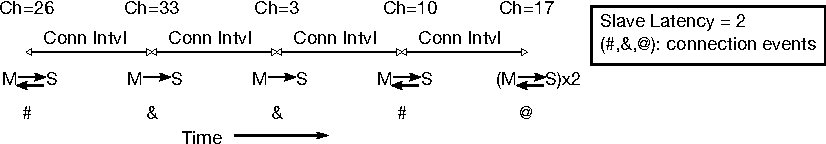
\includegraphics[scale=1.1]{ConnIntvl.pdf}
\caption{Illustration of BLE connection parameters}
\label{fig:ConnIntvl}
\end{figure}

An illustration of these parameters is presented in figure \ref{fig:ConnIntvl}. In this figure the concept of connection event, connection interval, slave latency, frequency hopping, hop increment and channel map can be visualized. The interaction that happens after every connection interval is the connection event as represented by `\#', `\&' and `@'. The slave latency considered in this example is 2. Its effect can be seen when the slave chooses not to respond to the master in the two `\&' connection events. But it \emph{had} to respond in the third connection event to keep the connection alive. Also it chose to respond in the `@' connection event. Multiple packets were communicated in this event by a mechanism described in the next paragraph. The frequency hopping can also be seen when the channel used changes for each connection event. The hop increment used in this example is 7. The working of the hopping algorithm can be seen when the channel hops from 33 to ((33+7)\%37), which is 3. The entire channel map is considered for this example. 


\begin{figure}[h]
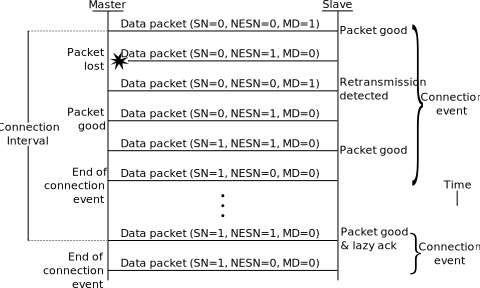
\includegraphics[width=0.9\textwidth]{SeqNum}
\caption{Illustration of working of BLE link layer's \gls{sn}, \gls{nesn} and \acrshort{md}}
\label{fig:SeqNum}
\end{figure}

Error detection in BLE communication is performed by utilizing 24 bit \gls{crc} in every packet. A simple acknowledgment scheme is used to request retransmission in case an error is detected or packet reception does not happen. This uses two bits called `\gls{sn}' and `\gls{nesn}'. When a device gets a packet with a particular \gls{nesn},  it must use that as \gls{sn} when it transmits a packet. In case a packet is missed, the device does not know \gls{nesn} and uses the old \gls{sn} in its transmitted packet, thus indicating that it did not receive the last packet. This is better illustrated in figure \ref{fig:SeqNum}. When the slave's packet is lost, the master uses the previous \gls{sn}, thus indicating retransmission. After that the \gls{sn} follows \gls{nesn}.

 
Another important parameter used in maintaining BLE connection is the `\gls{md}' bit. The \gls{md} bit indicates if a device has more data to send, so that more packets can be exchanged in a connection event. In figure \ref{fig:SeqNum}, the master has \gls{md} set to one while slave has it set to zero, indicating that the master has more data to send. In this case the master and slave exchange two packets in a connection event until both master and slave have \gls{md} as zero. In the second connection event, both master and slave have \gls{md} as zero, causing the connection event to end after exchange of one packet. \gls{md} bit allows communication of multiple packets in a connection interval when there is large amount of data to be communicated, thus increasing the throughput. This \gls{md} bit is used in the `@' connection event in figure \ref{fig:ConnIntvl} for two exchanges of packet.

\paragraph{\gls{l2cap}} This layer is responsible for multiplexing data from different logical channels in BLE, although in Bluetooth 4.0 only three fixed channels are used. 

\paragraph{Security Manager} This layer is used for pairing BLE devices, which is a form of authenticating the other device. Typically this is followed by encryption key distribution.

\paragraph{\gls{att}} This layer defines the \emph{Client-Server} architecture used by BLE to communicate data. A server is where data is held in a database and a client is one which gets the data from a server. All data stored in BLE devices as \emph{Attributes}, which is data organized in a specific format containing a label and address. Thus, a client can requests and gets a specific attribute from a server's database. Client or server configuration is independent of the role in link layer. A master or slave device can have \emph{both} a client and a server.

Attributes can be accessed from the attribute database in six ways as listed below.

\begin{easylist}[itemize]
& Find Requests: Client can find the attributes present in server's database.
& Read Request: Clients requests to get an attribute in server, to which the server responds with the requested attribute.
& Write Request: Client writes to an attribute in server with acknowledgment back.
& Write Command: Client writes to an attribute in server without acknowledgment back.
& Notification: Unprompted by the client, server sends an attribute to a client, to which the client does not acknowledge.
& Indication: Unprompted by the client, server sends an attribute to a client, to which the client acknowledges.
\end{easylist}

\paragraph{\gls{gatt}}
This layer organizes the attributes in a hierarchical manner, so that similar attributes can be encapsulated together. The hierarchical order from the top is as \emph{profile}, \emph{service}, and \emph{characteristic} i.e a profile contains one or more services, a service contains one or more characteristics and a characteristic contains one value and one or more descriptor. For example, a Time profile contains Current Time service, Next DST Change service and Reference Time Update Service. The Current Time service contains current time, local time and reference time characteristics. 

\paragraph{\gls{gap}}
This layer defines how BLE devices discover, connect and present useful information to the users and each other. A device having peripheral \gls{gap} role advertises and then connects to become a slave at link layer. A \gls{gap} central device initiates connection to a peripheral and becomes a master at link layer once connected.

\section[Overview of Contiki \texorpdfstring{\gls{os}}{OS}]{Overview of Contiki \texorpdfstring{\gls{os}}{OS}} \label{OverviewContiki}

Contiki \gls{os} is a lightweight, mature and open source operating systems with extensive networking stack for low cost and low power systems\cite{Contiki}. In this document `Contiki' and `Contiki \gls{os}' have been used interchangeably and mean the same thing. Contiki's networking capabilities include the complete IP stack (IPv4, IPv6, UDP, TCP, HTTP) and the recent \gls{ietf} standardized protocols for IPv6 networking such as RPL multihop routing protocol, 6LowPAN and CoAP RESTful application layer protocol. For the event driven scheduler that Contiki uses, a mechanism called \emph{Protothreads} is used. This results in low memory foot-print and nice flow control in code development. Another tool developed to ease development using Contiki, especially in large distributed systems is \emph{Cooja}. Cooja is a network simulator that has the capability of simulating large scale network on emulated hardware units with fine grained control. Cooja was used in this thesis also to verify designed before actually deploying them. Low power \glspl{wsn} is the typical application scenario of devices running on Contiki, although Contiki has been used in a wide variety of projects.



\subsection{Porting the Contiki to a New Platform} \label{2Porting}
Contiki \gls{os} has been ported to an increasing number of hardware platforms \cite{contikiHw}. Since Contiki is an open-source BSD Clause-3 licensed project, there are many projects in various hardware platforms based on a fork from the Contiki repository.

These hardware platforms' processors range across a spectrum of 8-bit (8051 and AVR), 16-bit (MSP430) to 32-bit (ARM Cortex-M, PIC32). Contiki has support for 802.15.4 based wireless communication with various external transceivers and \glspl{soc} with radio transceiver built in the same \gls{ic} as the \gls{mcu}. Various common features of many platforms such as \glspl{led}, buttons and serial port have modules in Contiki for common \gls{api} across platforms.

In \cite{Oikonomou2011} the authors describe Contiki's port to a CC2430 based platform manufactured by Sensinode Ltd. CC2430 is an enhanced Intel 8051 processor based \gls{soc} having 802.15.4 physical layer compatible radio transceiver. The authors fully debugged the port which had of a code footprint of about 100 kB, varying based on the compiler mode and the features enabled. Many new features were added to the port including support for \gls{adc} unit, all the sensor available on the platform (accelerometer, light sensor, voltage and temperature sensors), watchdog timer and the general purpose buttons. Because of the limited stack availability of 233 bytes, many optimizations such as moving variables to external \gls{ram} memory space and re-writing the radio driver for CC2430 to prevent stack from overflowing.

Contiki was ported to two new platforms, namely MicaZ and TelosB in a Bachelor thesis \cite{stan2007porting}. TelosB, similar to the TMote-Sky platform, consists of a 8MHz 16-bit MSP430 \gls{mcu}, a CC2400 transceiver with 802.15.4 \gls{phy} and a host of sensors to measure light, temperature and humidity. The port to TelosB was done by changing the port to the fully supported TMote-Sky platform. MicaZ platform consisted of a 8-bit Atmel ATMega128L \gls{mcu} and a CC2400 transceiver. MicaZ platform needed rewriting of the code for processor abstraction so that the high level Contiki \glspl{api} could work.

Contiki has been ported into platform based on a ARM Cortex M3 processor to create a device wired with Ethernet to connected to the Internet \cite{Wilde2013a}. Ethernet based networking with the libraries present in Contiki was developed in this project to demonstrate as a proof of concept. There are many unofficial ports of Contiki to various hardware platforms.

\section{Overview of 802.15.4} \label{Overview15.4}
802.15.4, maintained by IEEE 802.15 group, is a standard for the physical and \gls{mac} layer for low data rate wireless network\cite{IEEE802154}. Mnay protocols such as Zigbee and WirelessHART are based on 802.15.4. The emphasis of this protocol is to provide low cost, low power, low data rate wireless communication for short range, which is similar to \gls{ble}. One of the differentiating factors from \gls{ble} is that many of the protocols based on 802.15.4 support multi-hop. This expands the applications supported by 802.15.4 networks, especially when the application requires machine to machine communication.

Following the research community which primarily uses many different \gls{mac} layers in favor of the standardized 802.15.4 \gls{mac} layer, this thesis uses ContikiMAC and Null-RDC layers along with the physical layer of 802.15.4. Both ContikiMAC and Null-RDC are natively supported in Contiki across various platforms. In this report unless mentioned otherwise, 802.15.4 is implied to be using either ContikiMAC or Null-RDC, not the standard 802.15.4 \gls{mac}.

\subsection{Physical Layer}
\begin{figure}[h]
\centering
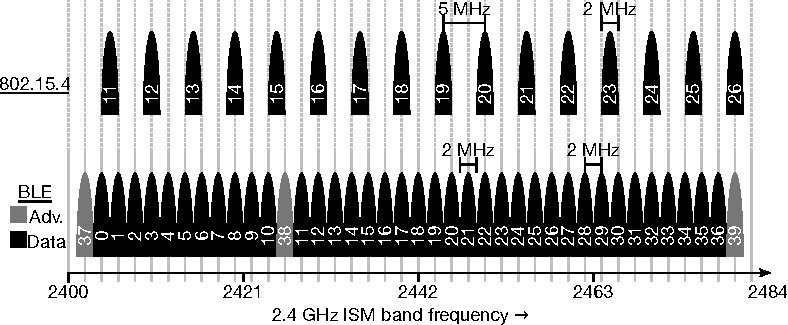
\includegraphics[scale=1.15]{ChMap_BLE_15_4.pdf}
\caption{BLE and 802.15.4's channel map comparison}
\label{fig:ChMap}
\end{figure}

802.15.4 also uses the 2.4 GHz \gls{ism} band for communication, with this spectrum divided into 16 channels numbered from 11 to 26. The bit rate used for this standard is 250 kbps. The modulation scheme used in 16-ary orthogonal modulation using Direct Sequence Spread Spectrum technique. 0 to 10 channels of 802.15.4's are present in sub 1 GHz bands with lower bit rate. Comparison of BLE and 802.15.4's channel map is presented in figure \ref{fig:ChMap}.

\subsection{\texorpdfstring{\gls{mac}}{MAC} Layer}

Unlike BLE where the communicating nodes in a connection are tightly synchronized, the nodes operate asynchronously with 802.15.4. This is done by the nodes periodically switching on their receivers to sense any radio activity using the \gls{rssi} measurement. If any activity is sensed, the radio is kept on longer to enable reception if a packet is sent. The sender on the other hand transmits a number of strobe packets to inform the receiver that it is being sent a packet. Since these strobe packets contain the address of the intended receiver, the other neighboring devices can go back to sleep after receiving a strobe packet. The duration of sending these strobe packets must be longer than the sleep interval of all the neighboring nodes so that they won't miss the strobes.

A mechanism called \gls{cca} is used by the senders to ensure that the channel is free before initiating communication i.e. sending the strobe packets. This is done since process of sending strobes aggressively occupies the channel, so it is important to verify that the channel is clear. This is again done with \gls{rssi} measurement.

\begin{figure}[h]
\centering
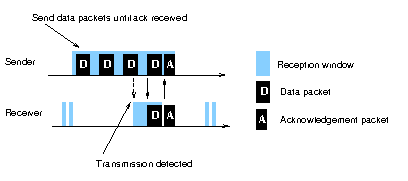
\includegraphics[scale=2,trim={0cm 0.1cm 0cm 0.3cm}]{ContikiMAC.pdf}
\caption{Working of ContikiMAC \cite{Dunkels2011}}
\label{fig:ContikiMAC}
\end{figure}

This mechanism is also followed in ContikiMAC with some additional optimizations such as fast wake-up and phase lock for lower power consumption. The process of strobing in case of ContikiMAC is done with data packets as shown in figure \ref{fig:ContikiMAC} from \cite{Dunkels2011}. The default wake up interval of the nodes with ContikiMAC is 125 ms. In case of Null-RDC the radio receiver is never switched off, as the name suggests. Null-RDC also uses the \gls{cca} mechanism to check if the channel is free before sending strobe packets.
